\documentclass[11pt]{article}
\usepackage[margin=1.15in]{geometry}
\usepackage{amsmath,amssymb,amsthm,booktabs,graphicx,natbib,hyperref,setspace}
\graphicspath{{../outputs/figures/}}
\onehalfspacing
\newtheorem{proposition}{Proposition}
\title{Persistent Records and Rehabilitation Incentives}
\author{Aayush Kadam}
\date{September 2026 --- Working Paper, External Review Version v0.1.0}

\begin{document}
\maketitle

\begin{abstract}
Past behavior can predict future behavior and discipline current actions. When agents can invest in changing their future productive state, however, a persistent public record also changes the return to that investment. I study a finite-horizon dynamic control problem that separates persistence of an institutional score from persistence of underlying quality. On a nonempty region, greater score persistence strengthens ex ante discipline while reducing productive effort after an adverse history. Records can consequently produce differences in future quality rather than merely reveal them: even with zero intrinsic quality persistence, different records generate different next-period quality whenever they induce different effort. Repeated score-dependent effort can propagate these differences over a finite horizon. The feedback is regional. Depending on the local geometry of opportunity, an adverse record can suppress or stimulate effort, producing self-confirming and self-correcting regions. A secondary numerical exercise finds that lifecycle-contingent persistence can outperform a constant rule in parts of parameter space, but gains can be small and direct punishment can substitute for memory. The paper therefore establishes neither a universal case for forgetting nor a universal optimal record duration.
\end{abstract}

\section{Introduction}

Past behavior is useful because it forecasts future behavior and can discipline present actions. But a record is not purely informational when the person or firm being recorded can invest in changing future outcomes. Persistent adverse information lowers or delays future opportunity, changing the return to productive rehabilitation. The record can then help produce the future fundamentals it is used to forecast.

This paper studies that mechanism in a deliberately transparent setting. An institutional score $R_t$ summarizes public history, while a distinct productive state $x_t$ evolves with intrinsic persistence $\rho$ and productive effort $e_t$. The score persists at rate $\phi$. Opportunity is an increasing reduced-form function $A(R_t)$. A clean agent may take a privately beneficial harmful action; after an adverse event, the agent may invest in future quality. The environment is a finite-horizon control problem, not a Bayesian or competitive-market equilibrium.

The first contribution is a regional lifecycle-asymmetry result. Increasing the same score-persistence parameter can raise the expected consequence of misconduct before an adverse event and reduce the marginal return to productive effort afterward. The result holds globally for the interior linear-opportunity rehabilitation benchmark and on a characterized region under smooth nonlinear opportunity. It is not a global monotonicity claim.

The second contribution separates institutional from intrinsic persistence. When two agents have identical current fundamentals but different public records, record-dependent effort can generate different next-period quality. This channel operates even at $\rho=0$. Iterating the transition shows exactly how future quality gaps decompose into intrinsic carryover and a distributed lag of effort gaps. At zero intrinsic persistence, multi-period differences require repeated record-dependent effort.

The regional qualification is economically important. Under smooth opportunity, the response of effort to the inherited record depends locally on opportunity curvature. A worse record can lower effort and become self-confirming, but it can also raise compensating effort and become self-correcting. The model therefore does not imply that stigma is globally self-fulfilling.

The paper's design analysis is secondary. A finite computational exercise compares one constant persistence rate with a clean/adverse lifecycle rule. State contingency often has positive value in the tested design, but the benchmark gain is modest, some environments yield negligible gains, and costless direct sanctions can outperform memory alone. These results are reported as an appendix illustration rather than as a universal policy prescription.

\section{Related literature}

The mechanism sits at the intersection of reputation, endogenous quality, limited records, and dynamic sanctions. \citet{boardmeyer2013} study reputation when firms invest in endogenous persistent quality; \citet{bohren2024} shows how a persistent payoff-relevant state creates dynamic moral-hazard incentives. Those papers establish that reputation and persistence can affect real investment. The narrower object here is an institutional score-persistence parameter with opposed pre-event discipline and post-event productive-effort effects.

Work on limited and fading records shows that memory changes reputational incentives. \citet{liuskrzypacz2014} analyze limited records and reputation bubbles, while \citet{sperisen2018} compares bounded and fading memory. \citet{bhaskarthomas2019} show how bounded-memory punishment states sustain community enforcement. \citet{elulgottardi2015} analyze regulated forgetting in credit markets. These contributions preclude a novelty claim for bounded memory, temporary punishment, or welfare-improving forgetting themselves.

Record erasure and direct instruments provide additional close benchmarks. \citet{pei2026} studies strategic deletion of records. \citet{jovanovic2021} models product recalls and shows that a recall tax with a subsidy can attain the first best in that environment. The analysis below consequently treats memory as a constrained institutional instrument rather than a uniquely optimal sanction.

The distinction from this literature is modest and specific: the same score persistence governs a pre-event deterrence margin and a post-event investment margin in a model that separates score memory from underlying-state memory. The paper does not claim priority for reputation-dependent investment, fading memory, forgiveness, or state-contingent punishment.

\section{Environment}

Time is discrete and finite, $t=0,\ldots,T$. The public state is $(R_t,x_t,z_t)$, where $R_t$ is an institutional score, $x_t$ is underlying productive quality, and $z_t\in\{C,A\}$ denotes a clean or adverse lifecycle state. The score is not assumed to be a Bayesian posterior.

An institution maps the score into current opportunity $A(R_t)$, where $A$ is weakly increasing. In an adverse state the agent chooses productive effort $e_t\in[0,1]$ at cost $\kappa e_t^2/2$. Quality and the public signal evolve according to
\begin{align}
x_{t+1}&=\rho x_t+\alpha e_t+\varepsilon_{t+1},\\
y_{t+1}&=x_{t+1}+\eta_{t+1},\\
R_{t+1}&=\phi R_t+(1-\phi)y_{t+1}.
\end{align}
The parameters $\rho$ and $\phi$ are conceptually different. The first carries true quality forward; the second carries the institutional record forward. The parameter $\alpha$ converts effort into future quality.

The canonical within-period order is state observation, opportunity assignment, lifecycle-specific action, flow payoff, quality transition, signal, and score update. The opportunity schedule is reduced form. Short-lived market participants and belief consistency are not solved, so the model is a dynamic control problem rather than a Markov perfect equilibrium.

\section{Recovery and productive rehabilitation}

Suppose an adverse score $R_0<\bar R$ is followed by a constant favorable signal $y_G>\bar R$. The score path is
\[
R_t=y_G+\phi^t(R_0-y_G),
\]
and the continuous crossing time is
\[
n(\phi)=\frac{\log[(y_G-\bar R)/(y_G-R_0)]}{\log\phi}.
\]
For $0<\phi<1$, $n'(\phi)>0$. More persistent records delay recovery. In discrete time the first crossing is the corresponding weakly increasing integer step function.

For the productive-effort benchmark, let $x_1=\rho x+\alpha e$, $m=\phi^H$, and $r=mR+(1-m)x_1$. The adverse agent solves
\[
\max_{e\in[0,1]}\;\beta^H V A(r)-\frac{\kappa e^2}{2}.
\]
With an unclipped linear schedule $A(r)=a+br$, an interior solution is
\[
e^*(\phi)=\frac{\beta^H Vb\alpha(1-\phi^H)}{\kappa}.
\]
Thus persistence reduces productive effort whenever the solution is interior. Intuitively, placing more weight on the inherited adverse score reduces the effect of new quality on future opportunity.

For a twice differentiable increasing schedule, implicit differentiation gives
\begin{equation}
\frac{\partial e^*}{\partial\phi}=
\frac{\beta^H V\alpha H\phi^{H-1}\{-A'(r)+(1-m)A''(r)(R-x_1)\}}
{\kappa-\beta^H V[\alpha(1-m)]^2A''(r)}.
\label{eq:effortphi}
\end{equation}
At a strict interior optimum the denominator is positive. The first term in braces is attenuation of the new signal; the second relocates the agent along a curved opportunity schedule. Their sum need not have a common sign across states.

\section{Lifecycle asymmetry}

Before an adverse event, a clean agent receives private misconduct benefit $b$. Detection occurs with probability $p$ and sends the score to $R_{bad}$. Let the opportunity loss from the induced recovery delay be
\[
P(\phi)=V[1-\beta^{n(\phi)}].
\]
The agent commits misconduct when $b\geq pP(\phi)$. Because recovery time increases with $\phi$, the threshold rises with persistence. Misconduct therefore weakly falls and falls strictly away from support boundaries.

\begin{proposition}[Lifecycle asymmetry]
There exists a nonempty open set of clean and adverse states in which an increase in common score persistence $\phi$ strictly reduces misconduct by the clean agent and strictly reduces productive rehabilitation effort by the adverse agent.
\end{proposition}

\noindent\emph{Proof sketch.} Choose a clean state with an interior misconduct threshold. The preceding recovery argument makes misconduct strictly decreasing in $\phi$. Choose an adverse state with an interior linear-opportunity solution, or a smooth-opportunity state satisfying the strict negative numerator condition in equation \eqref{eq:effortphi}. Both inequalities persist under small parameter perturbations. Complete details are in the appendix.

The proposition is an existence result. Detection can be ineffective or punishment can saturate. Under nonlinear opportunity the relocation term can dominate attenuation and reverse the effort comparative static. The result is therefore a lifecycle tension, not a recommendation for uniformly short records.

\begin{figure}[t]
\centering
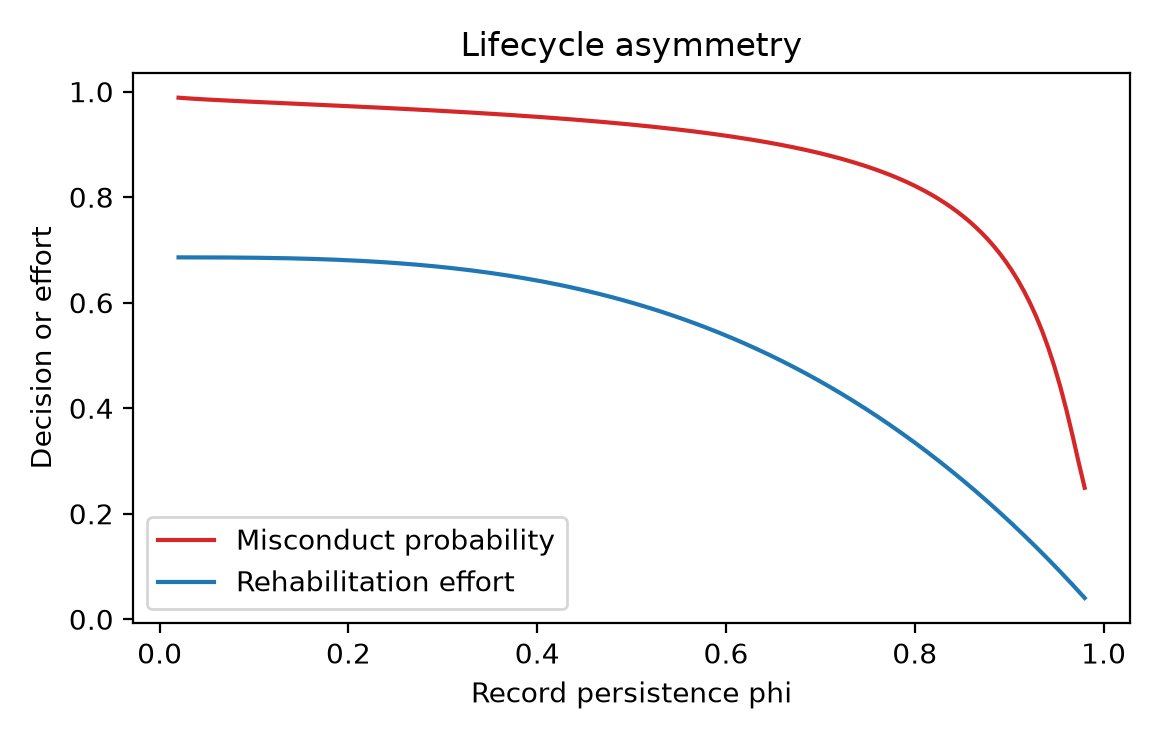
\includegraphics[width=.74\textwidth]{m1_lifecycle_asymmetry.png}
\caption{A benchmark lifecycle region. Greater persistence reduces both misconduct probability and productive post-event effort. The figure illustrates the proposition; it is not a calibrated policy estimate.}
\label{fig:lifecycle}
\end{figure}

\section{Institution-produced future outcomes}

Consider two histories, $A$ and $B$, with the same current quality and common future primitive shocks but different public records. Subtracting their quality laws gives
\[
\Delta x_{t+1}=\rho\Delta x_t+\alpha\Delta e_t.
\]
Iteration yields the exact identity
\begin{equation}
\Delta x_{t+h}=\rho^h\Delta x_t+
\alpha\sum_{j=0}^{h-1}\rho^{h-1-j}\Delta e_{t+j}.
\label{eq:gap}
\end{equation}
The first term is intrinsic propagation; the second is institutionally mediated behavioral propagation.

\begin{proposition}[Zero intrinsic persistence]
Set $\rho=0$ and $\alpha>0$. If two public records induce different effort at matched current fundamentals, then they generate different next-period true quality:
\[
\Delta x_{t+1}=\alpha\Delta e_t\neq0.
\]
At zero intrinsic persistence, a one-time effort difference lasts one period; a quality gap at later dates requires renewed record-dependent effort differences.
\end{proposition}

The proposition distinguishes a record's predictive content from its consequences. It does not say that all observed score predictiveness is causal, nor that the induced gap is permanent. It says that an institutional record can alter the process generating future quality even when current quality has no mechanical carryover.

\section{Self-confirming and self-correcting regions}

Let the local effort policy be differentiable, $e=e(x,R)$. The zero-shock transition Jacobian for $(x,R)$ is
\[
J_t=\begin{pmatrix}
\rho+\alpha e_x & \alpha e_R\\
(1-\phi)(\rho+\alpha e_x) & \phi+(1-\phi)\alpha e_R
\end{pmatrix}.
\]
At matched fundamentals, the immediate quality response to a record difference has the sign of $\alpha e_R$. If $e_R>0$, a worse record lowers effort and is locally self-confirming. If $e_R<0$, a worse record raises effort and is locally self-correcting.

In the strict-interior one-investment problem,
\[
e_R=\frac{\beta^H V\alpha(1-m)mA''(r)}
{\kappa-\beta^H V[\alpha(1-m)]^2A''(r)}.
\]
Hence the sign follows $A''(r)$. For logistic opportunity the boundary is the inflection point. Action bounds create flat regions, and nonconcavity can require global comparison.

\begin{figure}[t]
\centering
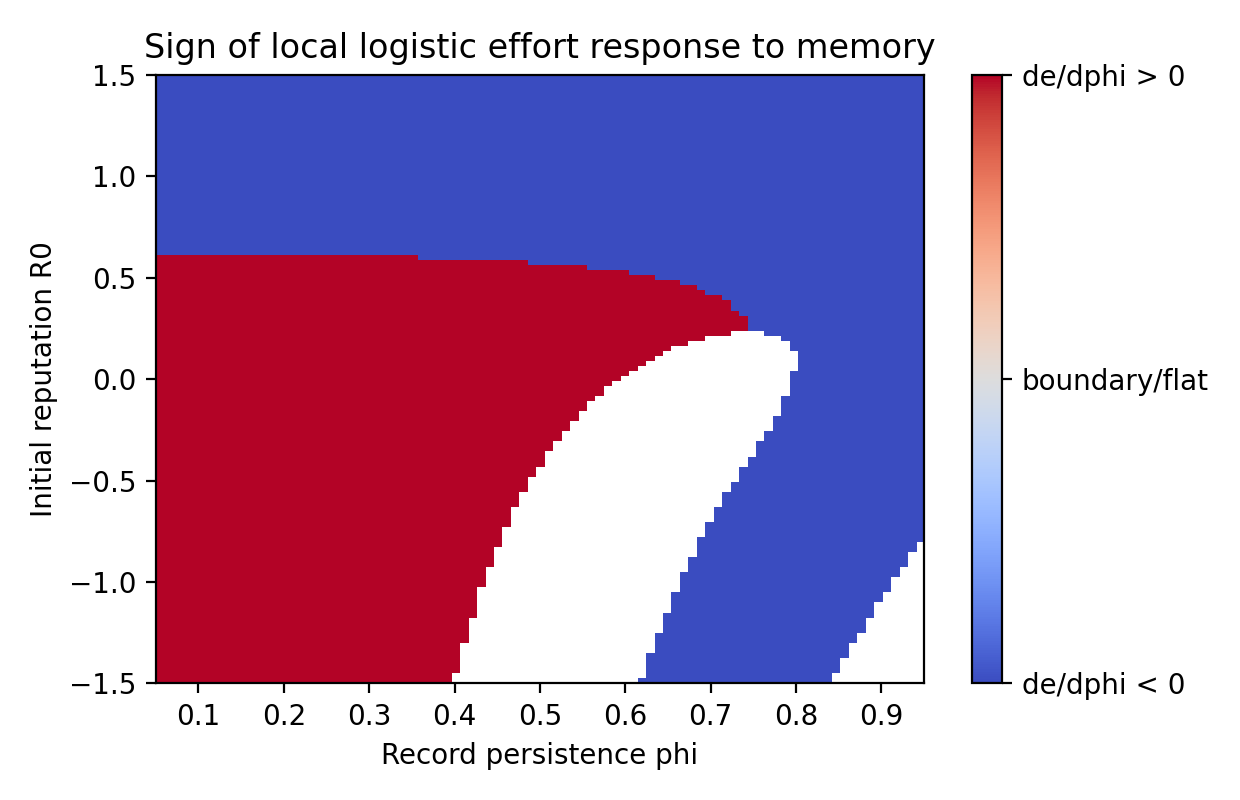
\includegraphics[width=.72\textwidth]{m1_5_logistic_sign_map.png}
\caption{Regional effort response under logistic opportunity. Both signs occur; white cells are boundary or flat solutions.}
\label{fig:regions}
\end{figure}

This regional structure rejects a global self-fulfilling-stigma theorem. The economic response to an adverse record depends on where the record places the agent on the opportunity schedule and on whether additional effort can move the score through a high-return region.

\section{Discussion and applications}

The model can describe institutional scores in credit, employment, online platforms, or professional records. In each case $R_t$ is a public summary, $A(R_t)$ maps that summary into opportunity, and $e_t$ is an investment that changes future productive capacity. The mapping is illustrative; no empirical calibration or legal prescription is offered.

The reduced-form opportunity schedule is the central limitation. A Bayesian market could infer current quality from both the score and endogenous effort, changing the opportunity map. An infinite-horizon equilibrium could also alter terminal incentives. False adverse signals are especially important because a persistent erroneous record may change the real state it initially measured incorrectly. These extensions require a different model rather than cosmetic robustness checks.

Direct instruments matter for interpretation. If fines, monitoring, or contracts are costless and unconstrained, record persistence need not be the preferred incentive device. Memory design becomes relevant when direct sanctions are legally, informationally, or financially constrained, or when the record serves a genuine screening role. Those constraints are not modeled here and should be objects of future work.

\section{Conclusion}

Public memory has informational and incentive consequences. A record summarizes history, but when opportunity depends on the record and effort changes future quality, the record also changes the return to becoming better. The resulting lifecycle tension is regional: persistence can strengthen discipline before an adverse event while weakening productive effort afterward, yet nonlinear opportunity can reverse the latter effect in other states.

Separating score persistence from intrinsic quality persistence clarifies the mechanism. Even at zero intrinsic persistence, different records can create different next-period fundamentals through effort. Repeated record-dependent choices can propagate those differences, but neither permanence nor globally self-confirming feedback follows.

The analysis does not identify a universal optimal half-life or a general case for forgetting. Its narrower lesson is that a record institution cannot be evaluated solely by how well it summarizes the past when it also changes the production of future outcomes. Empirical identification, Bayesian market responses, infinite-horizon incentives, and design under realistic constraints on direct sanctions remain open.

\appendix
\section{Formal Results and Proofs}

Throughout, $R$ is an institutional score rather than a Bayesian posterior. Let $\phi\in[0,1]$ be score persistence, $\rho\in[0,1]$ intrinsic quality persistence, and $\alpha\geq0$ effort productivity.

\subsection{Canonical finite-horizon control problem}
The state is $s_t=(R_t,x_t,z_t)$, where $z_t\in\{C,A\}$ denotes clean or adverse lifecycle status. In an adverse state the agent chooses $e_t\in[0,1]$ and
\[
x_{t+1}=\rho x_t+\alpha e_t+\varepsilon_{t+1},\qquad
y_{t+1}=x_{t+1}+\eta_{t+1},\qquad
R_{t+1}=\phi R_t+(1-\phi)y_{t+1}.
\]
Given an exogenous increasing opportunity schedule $A(R)$, the adverse-state Bellman equation is
\[
V_t^A(R,x)=\max_{e\in[0,1]}\left\{vA(R)-\frac{\kappa e^2}{2}
+\beta\mathbb E[V_{t+1}^A(R',x')]\right\}.
\]
In the clean state a private benefit $b$ is compared with the detection-weighted loss from transition to the adverse state. This is a dynamic control problem, not a market equilibrium.

\subsection{Proposition 1: recovery dynamics}
\textbf{Proposition 1.} If $R_0<\bar R<y_G$ and $0<\phi<1$, then under $R_{t+1}=\phi R_t+(1-\phi)y_G$,
\[
R_t=y_G+\phi^t(R_0-y_G),\qquad
n(\phi)=\frac{\log[(y_G-\bar R)/(y_G-R_0)]}{\log\phi},
\]
and $n'(\phi)>0$.

\textit{Proof.} Iteration gives the path. Direct differentiation gives
$n'(\phi)=-\log q/[\phi(\log\phi)^2]>0$ for $q\in(0,1)$. \qed

\subsection{Proposition 2: binary rehabilitation}
\textbf{Proposition 2.} Suppose rehabilitation costs $C$, yields value $V$ upon recovery, and $0<\beta<1$. If $C/V$ lies strictly between the endpoint values of $\beta^{n(\phi)}$, a unique threshold $\bar\phi(R_0)$ exists such that rehabilitation occurs below it and not above it.

\textit{Proof.} Proposition 1 and discounting imply that $\beta^{n(\phi)}V$ is continuous and strictly decreasing. Existence and uniqueness follow from the intermediate value theorem. \qed

When $y_G=\rho x+\alpha$, the threshold rises with $\alpha$ and $\beta$ and falls with $C$, wherever the derivatives exist.

\subsection{Proposition 3: continuous rehabilitation}
Let $m=\phi^T$, $x_1=\rho x+\alpha e$, and $r=mR+(1-m)x_1$. Consider
\[
U(e)=\beta^T V A(r)-\kappa e^2/2.
\]
\textbf{Proposition 3.} For linear $A(r)=a+br$, an interior optimum satisfies
\[
e^*=\frac{\beta^T Vb\alpha(1-\phi^T)}{\kappa},
\]
so $e^*$ strictly decreases in $\phi$. For twice differentiable increasing $A$, at a strict interior optimum,
\[
\frac{\partial e^*}{\partial\phi}=
\frac{\beta^T V\alpha T\phi^{T-1}\{-A'(r)+(1-m)A''(r)(R-x_1)\}}
{\kappa-\beta^T V[\alpha(1-m)]^2A''(r)}.
\]
Hence effort falls precisely where the numerator is negative.

\textit{Proof.} The first-order condition is $\beta^TV\alpha(1-m)A'(r)-\kappa e=0$. Differentiate implicitly and use the strict second-order condition. \qed

\subsection{Proposition 4: clean-state deterrence}
\textbf{Proposition 4.} Let detected misconduct cause recovery delay $n(\phi)$ and loss $P(\phi)=V[1-\beta^{n(\phi)}]$. A clean agent with benefit $b$ commits misconduct iff $b\ge pP(\phi)$. Thus the misconduct threshold rises with $\phi$; for a continuous benefit distribution, misconduct probability weakly falls and falls strictly away from support boundaries.

\textit{Proof.} Proposition 1 gives $P'(\phi)>0$. The remaining claims follow from the threshold rule. \qed

\subsection{Proposition 5: lifecycle asymmetry}
\textbf{Proposition 5.} There exists a nonempty set of clean and adverse states in which increasing the common score persistence $\phi$ strictly reduces misconduct and strictly reduces productive rehabilitation effort.

\textit{Proof.} Choose a clean state with an interior benefit threshold in Proposition 4. Choose an adverse state with an interior linear-opportunity solution in Proposition 3; both inequalities are strict on open parameter sets. For smooth nonlinear opportunity, replace linearity with the strict regional inequality $-A'(r)+(1-m)A''(r)(R-x_1)<0$ and the strict second-order condition. \qed

\subsection{Proposition 6: record memory without state memory}
\textbf{Proposition 6.} Set $\rho=0$ and $\alpha>0$. If two public histories induce $e(R^A)\ne e(R^B)$, then identical initial fundamentals generate $x_1^A-x_1^B=\alpha[e(R^A)-e(R^B)]\ne0$.

\textit{Proof.} Substitute $\rho=0$ into the state transition. \qed

\subsection{Proposition 7: minimal behavioral persistence}
\textbf{Proposition 7.} Following a one-time effort difference and no later effort differences,
\[
x_t^A-x_t^B=\rho^{t-1}\alpha(e_0^A-e_0^B),\quad t\ge1.
\]
With $\rho=0$ the gap is one-period unless record-dependent effort recurs.

\textit{Proof.} Apply the linear state difference equation recursively. \qed

\section{Institution-Produced Outcome Persistence}

Consider two worlds $A$ and $B$ with common future primitive shocks. Subtracting their quality laws gives
\[
\Delta x_{t+1}=\rho\Delta x_t+\alpha\Delta e_t.
\]
Iterating establishes the exact finite-horizon decomposition
\[
\Delta x_{t+h}=\rho^h\Delta x_t+
\alpha\sum_{j=0}^{h-1}\rho^{h-1-j}\Delta e_{t+j}.
\]
The first term is intrinsic propagation; the second is behaviorally produced propagation. In particular, if current fundamentals match, all later quality divergence is generated by effort differences inside the model.

\subsection{Zero intrinsic persistence}

When $\rho=0$, $\Delta x_{t+h}=\alpha\Delta e_{t+h-1}$. Therefore a one-time effort difference lasts one period, while repeated score-dependent effort differences can generate nonzero quality gaps at every finite horizon. This is a possibility result, not a universal persistence theorem: fixed effort or $\alpha=0$ eliminates the quality gap.

\subsection{Local propagation}

For a differentiable policy $e=e(x,R)$ and state ordering $(x,R)$, the zero-shock transition has Jacobian
\[
J_t=\begin{pmatrix}
\rho+\alpha e_x & \alpha e_R\\
(1-\phi)(\rho+\alpha e_x) & \phi+(1-\phi)\alpha e_R
\end{pmatrix}.
\]
At matched fundamentals, the one-period effect of a record difference on quality has sign $\operatorname{sign}(\alpha e_R)$. Hence $e_R>0$ defines a locally self-confirming region for a bad record, $e_R<0$ a self-correcting region, and $e_R=0$ a locally flat region. Jacobian roots are finite-horizon propagation diagnostics and are not interpreted as infinite-horizon equilibrium stability conditions.

For the strict-interior one-investment problem in Proposition 3, implicit differentiation with respect to the inherited record gives
\[
e_R=\frac{\beta^T V\alpha(1-m)m A''(r)}
{\kappa-\beta^T V[\alpha(1-m)]^2A''(r)}.
\]
Under the strict second-order condition the denominator is positive, so the boundary between self-confirming and self-correcting regions is $A''(r)=0$. For logistic opportunity this is the midpoint $r=\bar R$. Action bounds and nonconcavity create additional flat or discontinuous boundaries.

\section{Secondary Computational Design}

For a finite horizon and population distribution $\mu$, define
\[
W(\phi)=\mathbb E_\mu\left[\sum_{t=0}^{T-1}\beta^t
\left\{q A(R_t)x_t-m A(R_t)(1-x_t)-\frac{\kappa e_t^2}{2}\right\}\right]
-\omega_C L d(\phi).
\]
The first term is real productive surplus, the second is real bad-match loss, the third is effort cost, and the final term is misconduct harm among the clean share $\omega_C$. Opportunity payments are transfers and omitted.

\subsection{Constant-memory benchmark and existence}

\textbf{Proposition.} Let $\phi\in[0,\bar\phi]$ for $\bar\phi<1$. If the primitive transition, opportunity, and payoff functions are continuous and the agent policy is unique and continuous in state and $\phi$, then an optimal constant memory exists.

\textit{Proof.} Finite composition and integration preserve continuity, so $W$ is continuous in $\phi$. The domain is compact; existence follows from Weierstrass. \qed

The uniqueness condition is substantive: action bounds and multiple private optima can kink or discontinuously select policies. The computational planner therefore uses a global grid and reports boundary and multiple-local-optimum cases rather than imposing differentiability or concavity.

\subsection{Designer ordering and counterexamples}

Constructive numerical examples yield both $\phi_{\rm pred}>\phi_{\rm welfare}$ and the reverse, as well as both $\phi_{\rm full}>\phi_{\rm fixed}$ and the reverse. Consequently neither prediction-focused retention nor behavior-ignorant retention has a global directional bias in this finite-horizon model.

\subsection{Lifecycle-contingent persistence}

Let the committed rule be $\Psi=(\phi_C,\phi_A,\phi_G,m)$ for clean, adverse, and favorable-streak states. Constant memory is the restriction $\phi_C=\phi_A=\phi_G$.

\textbf{Proposition.} On a finite common memory-action set, adaptive memory weakly dominates constant memory. If two positive-weight reachable states have different unique maximizing actions, the dominance is strict.

\textit{Proof.} Constant action vectors are feasible adaptive vectors, giving weak dominance. With distinct unique statewise maximizers, no common action attains both statewise maxima; positive weights make the resulting loss strict. \qed

In the calibrated repeated-event model, lifecycle contingency strictly improves welfare, but the restricted earned-forgetting rule collapses to constant memory. This numerical result supports state contingency, not a general theorem favoring accelerated post-rehabilitation forgetting.

\subsection{Finite computational design}

The computational design compares nested finite policy classes on a common memory grid. Weak dominance holds at all 36 predeclared points. Two-state clean/nonclean memory strictly improves on constant memory at 33 points, but the benchmark gain is small and three points show negligible value. Prediction-optimal memory is longer, shorter, or equal to welfare-optimal memory across different design regions. These are deterministic design frequencies rather than population probabilities or empirical estimates.

A proposed memory-conflict index, defined as dispersion in singleton-state local welfare slopes, has near-zero negative correlation with adaptive value and is rejected as an organizing sufficient statistic.
\subsection{Adversarial robustness and limitations}
The preregistered bounded battery re-optimizes constant and clean/adverse lifecycle-contingent persistence on a common memory mesh in 61 environments. Nesting holds throughout, but magnitudes range from economically negligible under linear access to large under a hard opportunity threshold. Representative bounded continuous effort solutions differ from a 501-point grid by less than $9.72\times10^{-4}$. The exercises do not establish timing invariance, robustness to stochastic false positives, or global continuous optimality of the memory vector. Accordingly, the computational evidence supports only a regional lifecycle-contingent persistence claim.


\bibliographystyle{plainnat}
\bibliography{references}
\end{document}
